\documentclass[10pt,a4paper,twocolumn]{article}

\usepackage[margin=1.75cm,columnsep=0.65cm]{geometry}
\usepackage[T1]{fontenc}
\usepackage[utf8]{inputenc}
\usepackage{lmodern}
\usepackage{microtype}
\usepackage{graphicx}
\usepackage{booktabs}
\usepackage{array}
\usepackage{amsmath}
\usepackage{xcolor}
\usepackage[hidelinks]{hyperref}
\usepackage{url}

\definecolor{navy}{HTML}{17365D}
\definecolor{teal}{HTML}{007C91}
\hypersetup{colorlinks=true,linkcolor=navy,citecolor=teal,urlcolor=teal}
\urlstyle{same}
\setlength{\parindent}{1em}
\setlength{\parskip}{0pt}
\raggedbottom
\renewcommand{\arraystretch}{1.12}

\title{\textbf{Reproducible Python-to-ESP8266 Transfer of a Compact Load-Forecasting and Residual-Decision Model: A Chronological Case Study}}
\author{Md. Fouad Iqbal\\
\small Electrical and Electronic Engineering Graduate\\
\small Chittagong University of Engineering \& Technology, Bangladesh}
\date{September 2026}

\begin{document}
\maketitle

\begin{abstract}
This paper studies a bounded question in edge machine learning: whether a compact forecasting computation and its residual-threshold decision can be transferred reproducibly from Python to a physical ESP8266. The case study uses 5,000 half-hourly rows from a public smart-meter-style dataset whose numeric variables are normalized and whose physical measurement provenance and inverse scaling are not documented. Six forecasting approaches were evaluated using a single chronological holdout and five expanding-window folds with 2,000 non-overlapping test predictions. The floating-point edge model achieved mean fold MAE $0.133858\pm0.004271$ in normalized target units. Its absolute-error difference from ordinary linear regression was not statistically distinguishable under the stated HAC/Holm procedure ($p_{\mathrm{adj}}=0.745$), while its difference from random forest was small but statistically distinguishable ($-0.001378$, $p_{\mathrm{adj}}=0.0345$). Five residual or isolation-based anomaly methods were compared only by agreement with publisher-supplied algorithmic labels; the best observed F1 was 0.462 for a split-conformal threshold, whereas the static p99 rule transferred to the device had recall 0.154 and F1 0.267. A nine-parameter standardized linear model was exported as C++ constants. Host C++ and physical ESP8266 executions reproduced all 933 held-out predictions and all 933 decisions, with maximum device difference $8.9\times10^{-8}$ normalized units. Thirty batches of 2,000 device predictions averaged $50.427\,\mu$s per prediction. Whole-firmware instruction RAM reached 92\%, making it the primary integration constraint. These findings establish numerical portability and measured model-kernel execution for one board and dataset; they do not establish calibrated electrical sensing, physical-energy accuracy, independent event detection, end-to-end latency, or energy efficiency.
\end{abstract}

\noindent\textbf{Keywords:} chronological load forecasting; ESP8266; TinyML; hardware-in-the-loop; numerical parity; residual thresholding; reproducibility

\section{Introduction}
Short-horizon load forecasting is commonly evaluated with recurrent networks, tree ensembles, or statistical baselines on household and building data \cite{shi2018pooling,kong2019lstm,aurangzeb2024bilstm}. Separately, prediction residuals and unsupervised models have been used to identify unusual consumption patterns \cite{liu2018scalable,utomo2020multitiered,hernandez2024daily}. Edge-oriented work has examined cloud--edge collaboration, federated split learning, and embedded energy analytics \cite{hu2020edge,li2024federated,kolosov2025instrumental}. Consequently, the broad combination of forecasting, anomaly investigation, and edge computing is established prior art.

The narrower reproducibility problem remains useful: a model that appears adequate in Python can still fail after feature reordering, preprocessing changes, numeric conversion, or device integration. This study therefore separates model quality from transfer correctness. It asks whether a deliberately small computation can preserve predictions and threshold decisions across Python, independently compiled C++, and a physical ESP8266, and what resource constraint becomes visible in the whole firmware.

The work addresses four research questions:
\begin{enumerate}
    \item How do compact and conventional forecasters compare under leakage-aware chronological evaluation on this normalized case-study dataset?
    \item How sensitive is supplied-label agreement to residual-threshold choice and anomaly-method design?
    \item Does generated C++ reproduce Python predictions and decisions over the complete 933-row holdout on both host and ESP8266 targets?
    \item What timing, RAM, instruction-RAM, and flash costs are observed for the specified firmware and board?
\end{enumerate}

The contributions are a reproducible chronological evaluation pipeline; an explicit threshold and anomaly-method sensitivity analysis; a generated, auditable C++ model with complete held-out parity checks; and a whole-firmware timing/resource report with clear claim boundaries. No claim of algorithmic novelty, calibrated smart-meter operation, or worldwide first is made.

\section{Related Work and Research Gap}
Deep recurrent models have improved household forecasting on larger, physically grounded datasets \cite{shi2018pooling,kong2019lstm,aurangzeb2024bilstm}. Prediction-based anomaly detection has also been evaluated online and in multitier edge architectures \cite{liu2018scalable,utomo2020multitiered}. Hernandez et al. studied activity-related anomalies using data from a commercial meter, providing event context absent from the present dataset \cite{hernandez2024daily}.

For embedded intelligence, Hu and Tang presented an IoT smart-metering edge architecture \cite{hu2020edge}; Li et al. demonstrated federated split learning across Cortex-M4 meters and edge computers \cite{li2024federated}; and Gajendran et al. used ESP8266 nodes for physical data acquisition while evaluating forecasting on computer hardware \cite{gajendran2026ihems}. Kolosov et al. combined calibrated high-frequency sensing with embedded energy disaggregation on substantially stronger platforms \cite{kolosov2025instrumental}. MLPerf Tiny and MCUNet provide stronger general benchmarking and deployment frameworks than this application-specific experiment \cite{banbury2021mlperf,lin2020mcunet}.

These studies prevent a broad novelty claim. The present study instead contributes a transparent, small-footprint transfer audit on an ESP8266: byte-level model state, complete row-wise Python/C++/device agreement, threshold-decision parity, and measured whole-firmware constraints. Its dataset evidence is weaker than studies using documented physical meters, and this limitation is treated as part of the result rather than hidden.

\section{Materials and Methods}
\subsection{Dataset identity and scope}
The analyzed CSV is version 1 of the Kaggle listing \emph{Smart Meter Electricity Consumption Dataset} \cite{kaggleSmartMeter2024}. Its SHA-256 fingerprint is \texttt{D48DF940FD29444F...D9D5F9DC88F588}. The table contains 5,000 rows and seven columns from 1 January through 14 April 2024 at 30-minute intervals. After constructing a seven-day lag, 4,664 rows remain. No missing cells, duplicate timestamps, or non-30-minute gaps were found.

The continuous columns lie approximately in $[0,1]$, but the listing does not provide inverse-scaling metadata or a primary measurement protocol. Accordingly, MAE, RMSE, thresholds, and numeric differences are reported only in normalized target units. The 5\% ``Abnormal'' labels are publisher-described algorithmic labels, not independently verified electrical events. They are used for method agreement comparisons rather than physical fault claims.

\subsection{Features and chronological evaluation}
The common predictor set comprises target lags 1, 2, 48, and 336 plus hour, day of week, month, and weekend indicator. Each lag references an observation available before its prediction timestamp. Six approaches were compared: lag-1 persistence, lag-48 seasonal naive, ordinary linear regression, random forest (200 trees, maximum depth 12, minimum leaf size 2), histogram gradient boosting, and a standardized linear edge model. Random seeds were fixed at 42 where applicable.

The single holdout uses 3,731 earlier rows for fitting and 933 later rows for testing. For the edge model, the earlier segment is divided into 2,984 fitting rows and 747 threshold-calibration rows. The expanding-window protocol contains five folds; each has 400 calibration and 400 test rows, yielding 2,000 non-overlapping test predictions. MAE, RMSE, and sMAPE are reported. Fold-level 95\% Student-$t$ intervals are descriptive because there are only five folds.

Paired absolute-error differences use a moving-block percentile bootstrap with 10,000 replicates and block length 48. A Diebold--Mariano-style mean loss-differential statistic uses a Bartlett Newey--West HAC variance with lag 48; five comparisons are Holm-adjusted. Statistical significance is not treated as evidence of cross-dataset generalization.

\subsection{Residual and isolation-based decisions}
The device rule compares absolute forecast residuals with the 99th percentile of 747 chronological calibration residuals, giving a threshold of 0.383026 normalized units. Sensitivity was evaluated at percentiles 90, 92.5, 95, 97.5, 99, and 99.5. Additional methods were a rolling-week p99 threshold, adaptive EWMA p99 threshold, split-conformal 95\% threshold, and Isolation Forest with 5\% contamination. Precision, recall, F1, confusion counts, and alert rate describe agreement with the supplied labels. The retrospectively best threshold is not proposed as a deployable operating point because choosing it on final test labels would bias evaluation.

\subsection{Model export and hardware-in-the-loop protocol}
The selected device computation is standardized linear regression with eight coefficients and one intercept. Together with eight means, eight scales, and one residual threshold, its core numeric state contains 26 FP32 values (104 bytes). Each standardized prediction contains eight subtractions, divisions, multiplications, and accumulation additions at source level. The generated header fixes feature order and constants; Random Forest and Isolation Forest are not claimed to run unchanged on the device.

Three evidence layers were kept separate: Python float64 reference evaluation; an independently compiled C++17 FP32 host executable; and physical ESP8266EX NodeMCU 1.0 replay. In the full hardware-in-the-loop (HIL) test, all 933 held-out vectors, Python predictions, and decisions were stored in program flash. The board recomputed predictions, residual decisions, forecasting metrics, and confusion counts. This replay validates arithmetic and integration but not live lag-buffer operation or sensor acquisition.

Pure model-kernel time was recorded as 30 batch averages, each over 2,000 predictions. Compiler summaries supplied whole-firmware RAM, instruction-RAM (IRAM), and flash-code use for normal and full-validation builds. These totals include the ESP8266 core, Wi-Fi, HTTP, serial reporting, and application code; they are not isolated model footprints. ThingSpeak HTTP responses demonstrate prototype telemetry continuity only. No calibrated sensing interface or mains connection was used.

\section{Results}
\subsection{Forecasting performance}
Table~\ref{tab:forecasting} summarizes the expanding-window experiment. The compact FP32 and ordinary linear models are numerically indistinguishable at the reported precision because they implement the same affine mapping with different serialization. Both outperform naive baselines on this dataset. The compact model's 1.02\% MAE difference relative to random forest is statistically distinguishable under the stated test, but the absolute difference is small and should not be generalized beyond this case study.

\begin{table*}[t]
\centering
\caption{Five-fold expanding-window forecasting results. MAE and RMSE use normalized target units.}
\label{tab:forecasting}
\footnotesize
\begin{tabular}{lcccc}
\toprule
Model & MAE mean $\pm$ SD & MAE 95\% CI & RMSE mean $\pm$ SD & Pooled sMAPE (\%) \\
\midrule
Compact edge linear (FP32) & $0.133858\pm0.004271$ & [0.128555, 0.139161] & $0.165970\pm0.004175$ & 40.354 \\
Linear regression & $0.133858\pm0.004271$ & [0.128555, 0.139161] & $0.165970\pm0.004175$ & 40.354 \\
Random forest & $0.135236\pm0.003713$ & [0.130626, 0.139846] & $0.167993\pm0.003135$ & 40.593 \\
Histogram gradient boosting & $0.140116\pm0.004235$ & [0.134857, 0.145375] & $0.174222\pm0.003543$ & 41.882 \\
Seasonal naive (lag 48) & $0.188809\pm0.008865$ & [0.177802, 0.199816] & $0.235346\pm0.008103$ & 57.707 \\
Persistence (lag 1) & $0.191500\pm0.006112$ & [0.183910, 0.199089] & $0.237066\pm0.007700$ & 58.497 \\
\bottomrule
\end{tabular}
\end{table*}

\begin{table*}[t]
\centering
\caption{Paired MAE comparisons against the compact FP32 model over 2,000 predictions.}
\label{tab:statistics}
\small
\begin{tabular}{lrrr}
\toprule
Comparator & Difference & Bootstrap 95\% CI & $p_{\mathrm{Holm}}$ \\
\midrule
Linear regression & $-6.82\!\times\!10^{-11}$ & [$-4.44,3.78$]$\times10^{-10}$ & 0.745 \\
Random forest & $-0.001378$ & [$-0.002490,-0.000180$] & 0.0345 \\
Hist. gradient boost & $-0.006258$ & [$-0.008475,-0.003911$] & $1.92\times10^{-7}$ \\
Seasonal naive & $-0.054951$ & [$-0.059999,-0.050036$] & $2.27\times10^{-97}$ \\
Persistence & $-0.057642$ & [$-0.062364,-0.052358$] & $1.77\times10^{-114}$ \\
\bottomrule
\end{tabular}
\end{table*}

\begin{figure*}[t]
\centering
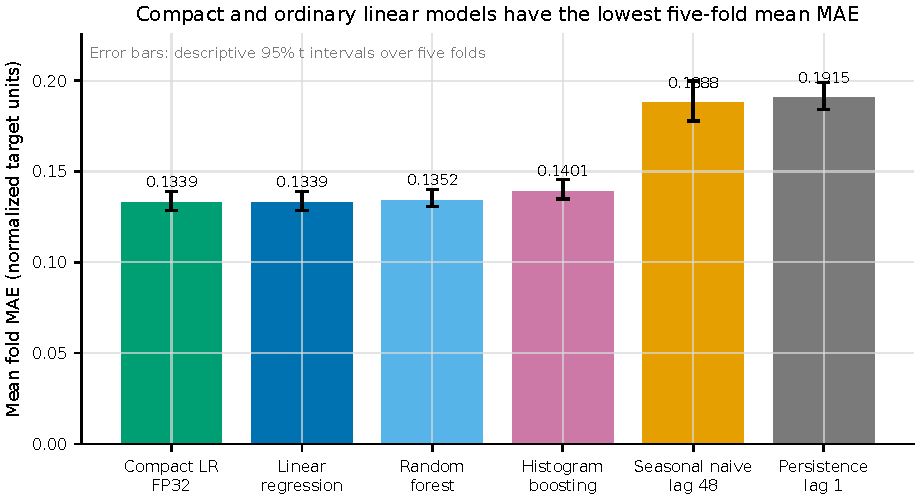
\includegraphics[width=0.92\textwidth]{../figures/fig03_forecasting_model_comparison.pdf}
\caption{Forecasting comparison using normalized target units. Error bars summarize fold-level variation; they do not establish performance on other datasets.}
\label{fig:forecasting}
\end{figure*}

Feature ablation produced mean MAE values from 0.133823 to 0.133890 across lag, calendar, and weather groupings. These small differences do not justify a claim that weather features drive forecasting performance. The eight-feature lag/calendar set was retained for deployment because it avoids external weather inputs while matching the tested alternatives closely.

\subsection{Anomaly-method and threshold sensitivity}
Table~\ref{tab:anomaly} shows that supplied-label agreement depends strongly on method and alert volume. Split conformal produced the highest observed F1 (0.462), while the deployed p99 rule generated no false positives but missed 44 of 52 supplied positives. At the retrospectively best static percentile (92.5), F1 reached 0.491 with 58 alerts; this is descriptive and was not used for the final device rule.

\begin{table*}[t]
\centering
\caption{Agreement with publisher-supplied algorithmic labels on the 933-row test segment.}
\label{tab:anomaly}
\small
\begin{tabular}{lrrrrrrrr}
\toprule
Method & TP & FP & FN & TN & Precision & Recall & F1 & Alerts (\%) \\
\midrule
Split conformal (95\%) & 21 & 18 & 31 & 863 & 0.538 & 0.404 & 0.462 & 4.18 \\
Adaptive EWMA p99 & 16 & 14 & 36 & 867 & 0.533 & 0.308 & 0.390 & 3.22 \\
Rolling-week p99 & 10 & 1 & 42 & 880 & 0.909 & 0.192 & 0.317 & 1.18 \\
Static residual p99 & 8 & 0 & 44 & 881 & 1.000 & 0.154 & 0.267 & 0.86 \\
Isolation Forest (5\%) & 19 & 114 & 33 & 767 & 0.143 & 0.365 & 0.205 & 14.26 \\
\bottomrule
\end{tabular}
\end{table*}

\begin{figure*}[t]
\centering
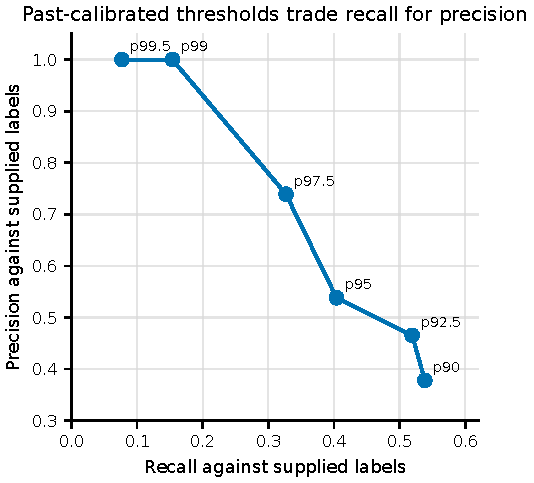
\includegraphics[width=0.92\textwidth]{../figures/fig05_anomaly_precision_recall.pdf}
\caption{Precision--recall behavior relative to the supplied labels. The labels are not independent physical anomaly ground truth.}
\label{fig:anomaly}
\end{figure*}

\begin{figure*}[t]
\centering
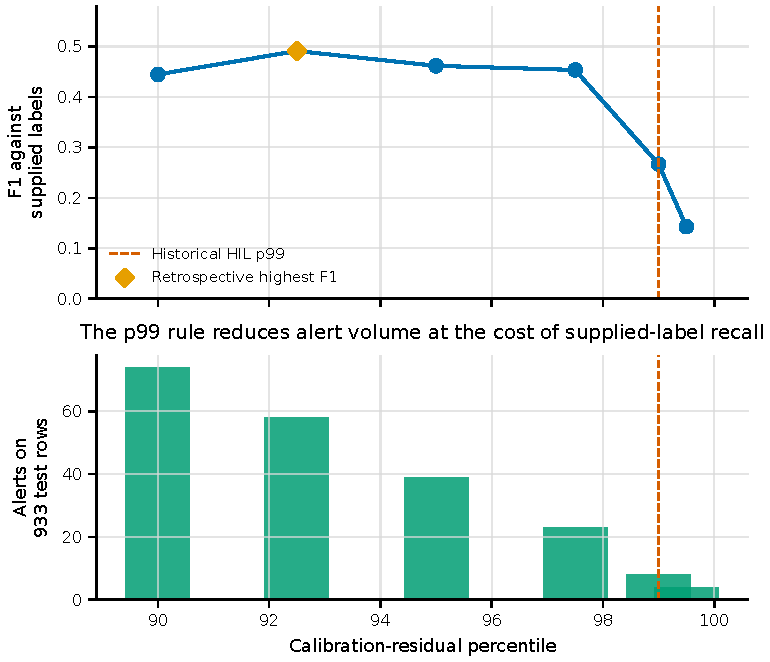
\includegraphics[width=0.92\textwidth]{../figures/fig06_f1_and_alerts_vs_threshold.pdf}
\caption{Static-threshold sensitivity. Lower thresholds increase label agreement and alert burden; selecting a threshold from these test results would bias a final evaluation.}
\label{fig:threshold}
\end{figure*}

\subsection{Cross-platform parity and embedded measurements}
The host C++ executable matched all 933 predictions and decisions, with maximum absolute difference $7.557\times10^{-8}$ normalized units. The physical ESP8266 also matched all 933 predictions and decisions; its maximum difference was $8.9\times10^{-8}$. Device-derived MAE, RMSE, and confusion counts matched the Python record within the declared tolerance. These results support numerical portability, not detector adequacy.

Across 30 batches, model-kernel timing had mean $50.427\,\mu$s, sample standard deviation $0.072\,\mu$s, median $50.403\,\mu$s, 95th percentile $50.539\,\mu$s, and range $50.362$--$50.700\,\mu$s per prediction. They are batch averages for one firmware/compiler/board setup, not individual-cycle, sensing-to-alert, or network-latency measurements.

\begin{table*}[t]
\centering
\caption{Python-to-device parity and whole-firmware resource evidence.}
\label{tab:embedded}
\small
\begin{tabular}{p{0.31\textwidth}p{0.25\textwidth}p{0.35\textwidth}}
\toprule
Measurement & Observed result & Claim boundary \\
\midrule
Host C++ prediction/decision agreement & 933/933; 933/933 & Generated-header arithmetic, not physical execution \\
ESP8266 prediction/decision agreement & 933/933; 933/933 & Flash-resident held-out replay, not live sensing \\
Maximum device difference & $8.9\times10^{-8}$ normalized units & Below the $10^{-4}$ parity tolerance \\
Kernel timing & $50.427\,\mu$s mean; 30 $\times$ 2,000 & Excludes sensing and communication \\
Normal firmware RAM / IRAM / flash & 29,516 / 60,343 / 257,796 bytes & 36.81\% / 92.08\% / 24.59\% \\
Validation firmware RAM / IRAM / flash & 29,852 / 60,343 / 298,132 bytes & 37.23\% / 92.08\% / 28.43\% \\
\bottomrule
\end{tabular}
\end{table*}

\begin{figure*}[t]
\centering
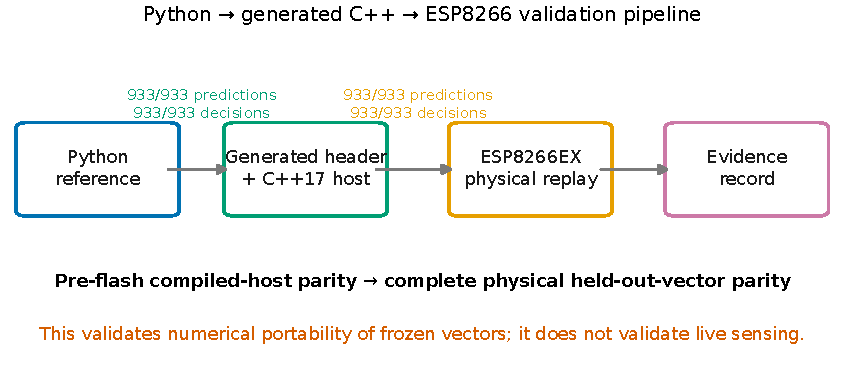
\includegraphics[width=0.92\textwidth]{../figures/fig07_python_cpp_esp8266_validation.pdf}
\caption{Evidence layers for Python, host C++, and ESP8266 execution. Complete parity applies to fixed held-out-vector replay.}
\label{fig:parity}
\end{figure*}

\begin{figure*}[t]
\centering
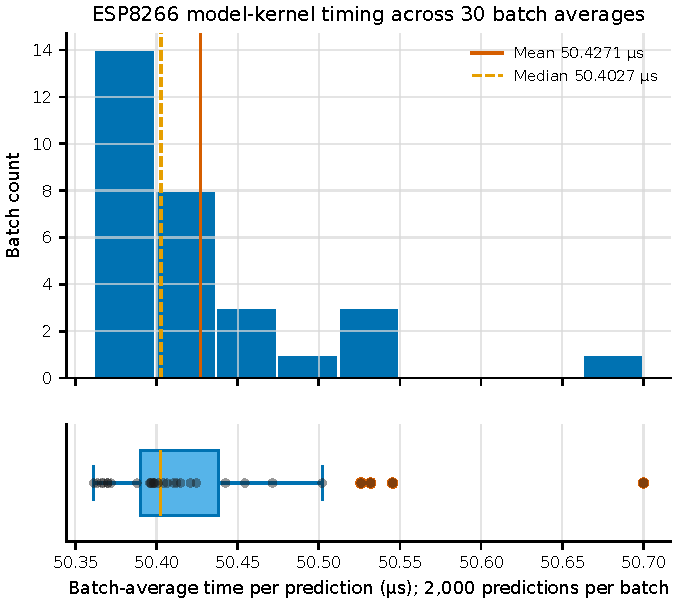
\includegraphics[width=0.49\textwidth]{../figures/fig09_esp8266_latency_distribution.pdf}\hfill
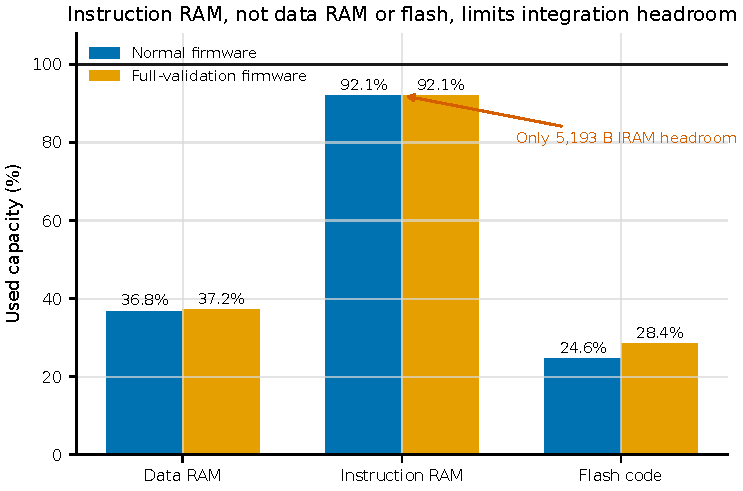
\includegraphics[width=0.49\textwidth]{../figures/fig10_memory_flash_iram_utilization.pdf}
\caption{Measured embedded costs: (left) distribution of 30 ESP8266 batch-average model-kernel measurements, each covering 2,000 predictions; (right) whole-firmware capacity use, showing IRAM as the principal measured integration constraint.}
\label{fig:embedded_costs}
\end{figure*}

Offline representation tests found identical decisions for standardized FP32, fused affine FP32, Q7/Q30, and Q15/Q30 forms over all 933 rows. Q15/Q30 reduced core coefficient/bias state from 104 bytes to 40 bytes (plus generic input-range metadata) with maximum deviation $1.211\times10^{-5}$ normalized units. Because physical fixed-point timing and whole-firmware measurements were not completed, the FP32 implementation remains the measured device result.

\section{Discussion}
The central result is the separation of forecasting evidence, label-agreement evidence, and deployment evidence. Chronological tests show that a compact affine model is competitive with the evaluated alternatives on this normalized dataset, but the similarity of feature-ablation results and the short 104-day span limit interpretation. The paired comparison against random forest is statistically distinguishable under the declared procedure, yet its absolute MAE difference is only 0.001378 normalized units. Simplicity is therefore justified here by portability and auditability rather than a broad accuracy claim.

The anomaly results are weaker. The static device threshold gives perfect precision only because it issues eight alerts and misses most supplied positives. The supplied labels themselves are not independent physical events. Thus neither the precision value nor the cross-platform decision agreement establishes reliable fault detection. Threshold sensitivity instead demonstrates the operational trade-off that must be revisited with verified events and prespecified selection rules.

Complete cross-platform parity is meaningful for implementation assurance. It rules out several common transfer failures over the tested holdout and confirms that the complete computation runs on the physical board. It does not show that the ESP8266 has received a calibrated load signal, maintained the 336-sample live history, or generated an operational forecast. The 92\% IRAM result also warns that adding TLS, signal processing, or sensing libraries may exceed this build's remaining instruction memory even though flash and general RAM have more headroom.

\section{Limitations}
The dataset has undocumented primary provenance, normalized values without inverse scaling, a short time span, and algorithm-generated anomaly labels. Only one dataset and one ESP8266 board were evaluated. The statistical procedure uses a prespecified one-day block/HAC lag and only five folds. The HIL experiment replays stored features instead of exercising a live lag buffer. Timing is a model-kernel batch average, and no end-to-end latency, current, power, or energy-per-inference measurement was made. The prototype telemetry uses HTTP and is not suitable for protecting credentials in field use. No independently calibrated voltage, current, power, or energy sensor was evaluated. These limitations prohibit claims of physical kWh accuracy, secure operation, energy efficiency, real-world anomaly performance, or general deployment readiness.

\section{Reserved ESP32 Field-Validation Extension}
\textit{This section is intentionally reserved. It will contain the sensor specification, isolation and conditioning circuit, calibration protocol, independently recorded reference measurements, field-data summary, event-labeling method, and ESP8266/ESP32 comparison only after those experiments are completed. No field result is claimed in the present version.}

\section{Future Work}
Future experiments should use an openly documented or independently collected meter dataset covering multiple seasons and verified events. The sensing stage must be isolated, reviewed, and calibrated against a trusted reference instrument before live-load claims. A timestamped circular buffer should be tested for startup, missing observations, clock drift, and restart recovery. Thresholds should be prespecified on training/calibration data and evaluated once on independent events. End-to-end sensing-to-alert latency, packet loss, current, power, and energy per inference should be measured. The security transport should migrate from prototype HTTP to certificate-validated HTTPS or authenticated MQTT. Finally, the Q15/Q30 candidate should undergo the same physical parity, timing, and whole-firmware resource protocol before any replacement decision.

\section{Conclusion}
This study demonstrates a reproducible method for transferring a compact forecasting and residual-decision computation from Python to a physical ESP8266. Across the complete 933-row held-out replay, host C++ and device execution preserved every prediction match and every threshold decision within sub-$10^{-7}$ normalized-unit difference. The board averaged $50.427\,\mu$s per prediction over 30 batches, while whole-firmware IRAM use reached 92\%. Chronological forecasting and anomaly comparisons provide context, but they do not convert the normalized dataset or publisher-supplied labels into calibrated physical evidence. The defensible outcome is therefore implementation fidelity with explicit resource and validity boundaries, not a new forecasting algorithm or a deployable smart meter.

\section*{Data and Code Availability}
Code, generated model constants, firmware, aggregate result records, split indices, figures, and reproduction instructions are provided in the public project repository. The raw third-party dataset and complete row-level validation vectors are not redistributed; the exact source URL, version, SHA-256 fingerprint, and regeneration procedure are documented. Private Wi-Fi and telemetry credentials are excluded.

\section*{Acknowledgment}
The author acknowledges the maintainers of the public dataset listing and the open-source Python, Arduino, ESP8266, and scientific-computing ecosystems used in the reproducibility workflow.

\clearpage
\bibliographystyle{IEEEtran}
\bibliography{../references/references}

\end{document}
